%\subsection{Основные особенности}
%Далее будут перечислены основные особенности предлагаемого языка:
В данном разделе будет представлен язык ЯЗ.
Основные особенности ЯЗ можно определить следующим образом:
\begin{enumerate}
\renewcommand{\labelenumi}{\theenumi.}
\renewcommand{\theenumi}{F\arabic{enumi}}


    \item ЯЗ является языком запросов, который позволяет осуществлять выборку по объектной 
    модели. %, определенной в~\cite{ODMG_3}.
%    \item ЯЗ позволяет преобразовывать выборку в необходимый для пользователя вид. 
%Данная возможность осуществима через вызов функции.
    \item\label{cut_query} ЯЗ самостоятельно выводит связи между объектами. 
%Для сокращения записи запроса язык предоставляет пользователю следующие возможности:
%	\begin{itemize}
%	
%	    \item не указывать связи между объектами (такие связи должны выводиться автоматически во время
%	выполнения запроса, например, строиться на основе метаинформации о модели);
%	    \item сокращать имена классов модели;
%	    \item сокращать сложные условия применяемые к одному свойству элемента.	    
%	\end{itemize}

    \item ЯЗ позволяет получать всю иерархию рекурсивных ссылок.
    \item ЯЗ предоставляет возможность вызова функции с данными из БД в качестве параметров. 
	Полученный от функции результат может стать результатом (или частью результата) запроса. 

\end{enumerate}

\subsection{Структура результата запроса}
Результатом запроса является:
    \begin{itemize}
	\item элемент, если структура результата состоит из одной структуры кортежа,
	    а запрос подразумевает один элемент в наборе кортежей в следующих случаях: 
	    \begin{itemize}
		\item кортеж результата содержит один элемент и выбирается только один кортеж;
		\item вызов функции как результата запроса 
		    (например, вызов функции суммирования по одному из свойств объекта).
	    \end{itemize}
	\item набор кортежей в любом другом случае.
    \end{itemize}

\subsubsection{Простая выборка}\label{simple-select}
Чтобы выбрать множество объектов заданного класса, достаточно задать имя класса:
\query{Room}
Данный запрос вернет пользователю множество объектов \cl{Room}.
Стуктура кортежа запроса состоит из одного элемента, типом
которого является класс \cl{Room}, поэтому каждый кортеж запроса
будет состоять из одного объекта класса \cl{Room}.
Если для класса не существует другого класса с таким же именем, но различным регистром
в написании всего имени или его отдельных букв (например, \cl{Room} и \cl{room}),
то для этого класса регистром можно пренебречь:
\query{room}

Также можно сокращать имена классов (в том случае если не возникает коллизий: 
например, если существует два класса, начинающиеся с буквы ``R'', то сократить
имя класса до ``r'' нельзя):
\query{r \\ro \\ roo}

Пользователь может самостоятельно определить сокращение для имени класса (механизм
задания таких сокращений определяется реализацией):
\query{rm}

Если сокращение пользователя для одного класса соответсвует одному из сокращений
другого класса, то в запросе должно подразумеваться сокращение пользователя.

Обращение к свойствам объекта необходимо производить через точку.  
Если необходимо выбрать свойство \cl{name} объекта \cl{Room}, 
то сделать это можно следующим образом:
\query{room.name}
В результат данного запроса будет включено значение свойства \cl{name} каждого объекта \cl{Room}.
Вложенность обращений неограничена:
\query{room.floor.building.name}

%Помимо свойства, ЯЗ позволяет возвращать значение результата выполнения метода объекта.
%Вызов его также осуществляется через точку, а результат выполнения включается в кортеж
%результата запроса. Параметры метода задаются через запятую в круглых скобках после
%имени метода. В том случае если метод не имеет параметров, то круглые скобки можно опускать.
%Метод не может ничего не возвращать. Если это происходить, то пользователь должен получить
%сообщение об ошибке. В преположении того, что метод \cl{getName} класса \cl{Room} возвращает
%значение свойства \cl{name}, то результат данного запроса
%\query{room.getName()}
%будет эквивалентен результату запроса
%\query{room.name}


Одной из особенностей ЯЗ является то, что ЯЗ пытается самостоятельно искать связи между 
объектами (подробнее см. в~\ref{tied_queries}). Поэтому в запросах на ЯЗ можно
сразу после точки указать имя другого класса, с которым неоходимо связать объекты.
В таком случае запрос
\query{room.networkinterface.inetAddress}
будет корректен и вернет значение свойства \cl{inetAddress} объектов \cl{networkinterface},
принадлежащих объектам \cl{room}. Корректность определяется тем, что между классами
\cl{Room} и \cl{NetworkInterface} существует связь, которая будет найдена
ЯЗ и применена для получения объектов \cl{networkinterface} для конкретно взятого
объекта \cl{room}.

Язык также предоставляет возможность обращения к коллекциям
элементов, при этом подразумевается, что такое обращение идет к объекту находящемуся в
коллекции, а не к самой коллекции.
Например, в таком запросе
\query{building.floors.number}
\cl{floors} представляет собой коллекцию, состоящую из объектов \cl{Floor}, поэтому
обращение \cl{.number} идет не к типу коллекции, а к типу элемента коллекции (т.е. к \cl{Floor}).
Данный запрос вернет номера (\cl{number}) этажей(\cl{Floor} из \cl{floors}), принадлежащих зданиям 
(\cl{building}).

Если необходимо выбрать несколько свойств объекта, то сделать это можно так:
\query{room[name number]}
Кортеж результата данного запроса будет состоять из двух элементов: для каждого объекта \cl{Room}
в результат будет включено значение свойства \cl{name} и \cl{number}.

Как следует из вышесказанного, через точку может задаваться как свойство, так и
имя класса другого объекта, с которым данный объект необходимо связывать. Реализация ЯЗ
должна осуществлять поиск отношения в соответствии со следующим списком приоритетов, расположенных в
порядке убывания: 
\begin{itemize}\addtolength{\itemsep}{-0.7\baselineskip}
    \item свойство;
%    \item метод;
    \item связь между двумя классами модели;
    \item поиск в наследниках или родителях (подробнее см. главу про полиморфизм).
% связь между наследниками и родителями .
\end{itemize}





\subsubsection{Выборка связанных элементов}\label{tied_queries}
Если необходимо выбрать связанные между собой объекты (предполагается, что между ними
существует связь на уровне модели), то необходимо задать связь, используя круглые скобки.
Например, запрос 
\query{building (room)}
на естественном языке можно сформулировать так: выбрать все здания (\cl{building}) и для каждого
здания показать список его комнат (\cl{room}). Скобки определяют следующий уровень иерархии
результата запроса (данный запрос имеет 2 уровня иерархии). Такой запрос возможен потому, что класс \cl{Building} связан с
классом \cl{Room} и существует возможность однозначно определить данную связь:
\cl{Building} имеет коллекцию \cl{floors}, состояющую из объектов \cl{Floor}, которые в 
свою очередь имеют коллекцию \cl{rooms}, состояющую из объектов \cl{Room}. Таким образом, 
для каждого объекта класса \cl{Building} имеется возможность найти множество принадлежащих ему
объектов класса \cl{Room}.
%В том случае если связь однозначно определить нельзя, то можно самостоятельно ее указать в запросе:
%\query{
    %building\#b (b.floor.room)
%    building (floor.room)
%}

%После имени класса через знак ``\#'' указано имя, на которое можно ссылаться далее
%по тексту запроса. Указание имени ссылки в данном случа обязательно, так как
%при таком запросе
%\query{building (building.floor.room)}
%или использовании любого другого сокращения
%\query{
%    building (b.floor.room)\\
%    building (buil.floor.room)
%}
%будет производиться поиск связи между объектами класса \cl{Building}.

Если невозможно найти связь между двумя указанными объектами, то пользователь должен
получить сообщение об ошибке. Если между объектами существует несколько
связей, то выбирается та связь, для которой требуется меньшее количество переходов по ссылкам.
Если существует несколько связей с одинаковой минимальной длиной переходов, то 
выбирается произвольная из этих связей.

Также существует возможность указания промежуточных звеньев связи:
\query{
    %building\#b (b.room.device)
    building (room.device)
}
С помощью данного запроса пользователь сможет получить список зданий(\cl{building}) и все 
принадлежащие ему устройства (\cl{device}). При этом он указывает, что эти устройства необходимо
искать у здания через комнаты (\cl{room}), т.е. сначала будет произведен поиск связи от здания
до комнаты, а потом от комнаты до устройств. Такая возможность может быть полезна при 
существовании нескольких связей между объектами. В этом случае можно идентифицировать
одну связь, указав промежуточное звено. 

Стоит обратить внимание, что поиск связи осуществляется по объектам классов модели, 
а не по их свойствам. Таким образом такие запросы будут некорректны:
\query{
    building (rooms)\\
    %building\#b (b.rooms.devices)
    building (rooms.devices)
}


Вложенность связей неограничена:
\query{building (room (device (networkinterface)))}
Кортеж данного запроса будет состоять из четырех элементов (запрос имеет четыре уровня иерархии): 
здание (\cl{building}), у каждого здания необходимо показать множество его комнат (\cl{room}), 
у каждой комнаты --- множество устройств (\cl{device}), 
а у каждого устройства --- множество его сетевых интерфейсов (\cl{networkinterface}).

Язык позволяет определять несколько типов элементов на одном уровне иерархии. Например,
такой запрос
\query{building (room, device)}
вернет список зданий, а для каждого здания список его комнат и устройств. При этом
в кортеже результата данного запроса будет всего два элемента. Второй элемент будет
либо комнатой (\cl{room}), либо устройством (\cl{device}). Поиск связи будет производиться
независимо два раза: от здания до комнаты и от здания до устройства.

В случае с несколькими элементами на одном уровне иерархии и последующим связыванием
следует придерживаться следующего правила: элемент на следующем уровне иерархии 
привязывается к последнему элементу предыдущего уровня иерархии. Таким образом,
в запросе
\query{builidng (room, simpleou (device))}
список устройств (\cl{device}) будет формироваться относительно простых
организационных единиц (\cl{simpleou}).

Еще примеры:
\queryexpl{\cl{floor} привязывается к \cl{room}}{building.device.room (floor)}
\queryexpl{\cl{floor} привязывается к \cl{device}}{(building.device).room (floor)}
\queryexpl{\cl{floor} привязывается к \cl{building}}{(building).device.room (floor)}




\subsubsection{Объединение запросов}
ЯЗ позволяет объединять результаты запросов в одном запросе. Объединение запросов 
выполняется при помощи запятой. Таким образом, объединение запросов представляет
собой задание нескольких структур кортежей на первом уровне иерархии. Например, запрос
\queryexpl{Получить все здания и комнаты}{building, room}
вернет список объектов \cl{Building} и \cl{Room} (результат см. в~\ref{ex_3}). 

Структура объединенных запросов может быть различна. Там где значение не определено, 
результат запроса должен содержать значение NOT\_DEFINED (в ЯЗ4J для обозначения
такого значения используется \cl{NOT\_DEFINED} перечисления \cl{Definitions}.).
Например, в запросе
\query{building (room), floor}
структура первого запроса отличается от структуры второго запроса (результат его выполнения
см. в~\ref{ex_5}). Первый запрос возвращает кортежи с двумя элементами, а второй --- с одним.

%Приведем еще несколько примеров:
%\query{building (room (device), device)}
%В данном запросе кортеж состоит из трех элементов.






\subsubsection{Выборка объектов по рекурсивным ссылкам}
Предположим, что у нас есть класс {\it Person}, описание структуры которого на псевдокоде выглядит так:
\begin{verbatim}
    class Person {
        String name = "";
        String surname = "";
        Person father = null;
        Person mother = null;
        Set<Person> children = new HashSet<Person>();
    }
\end{verbatim}
Данный класс имеет поля \cl{father} и \cl{mother}, которые также имеют тип \cl{Person} и поле-коллекцию
\cl{children}, состоящую из объектов типа \cl{Person}, которые в свою очередь также будут иметь
поля \cl{father},  \cl{mother} и \cl{children} и так далее. Как в таком случае получить всю 
иерархию объектов, например, по полю \cl{father}? Для этого в ЯЗ введены специальные
модификаторы, которые позволяют это сделать:
\query{person.father*}
или
\query{person.father+}
Оператор \cl{+} отличается от \cl{*} тем, что при \cl{+} в результат запроса будут
включены только объекты \cl{father}, тогда как при \cl{*} в результат также 
попадет сам объек \cl{person}.

Запрос с \cl{+} для каждого объекта \cl{person} найдет объект \cl{person.father} и включит
его в кортеж результата. Если найденный объект не представляет
из себя пустое значение, то будет найден объект \cl{person.father.father}, который будет 
включен следующим элементов кортежа. Такой поиск будет происходить до тех пор, пока не будет
найдено пустое значение. 
При запросе с \cl{*} в результат запроса сначала будет включен сам объект \cl{person}. 
Затем для этого объекта будет найден объект \cl{person.father}, который станет
следующим элементом кортежа. Если \cl{person.father} не равен пустому значению, то будет найдет
\cl{person.father.father} и включен в результат и так далее.

Если необходимо включать не сам объект \cl{person.father}, а, 
одно из его свойств, например, поле \cl{name}, то это можно сделать следующим образом:
\query{person.father*.name}

Модель на рис.~\ref{fig:son-model} также имеет рекурсивные ссылки: 
класс \cl{AbstractOU}, наследниками которого являются классы \cl{CompositeOU} и \cl{SimpleOU},
содержит поле \cl{parent}, имеющее тип \cl{CompositeOU}. Таким образом, чтобы для каждого 
\cl{SimpleOU} получить все его вышестоящие подразделения необходимо выполнить следующий запрос:
\query{simpleou.parent+}

Для примера организационной модели, приведенного на рис.~\ref{fig:model-snapshot-org}, 
данный запрос вернет следующий результат:\footnote{Если элементом результата запроса 
является объект, то в таблице с результатом приводится его строковое представление.}


\begin{center}
    \begin{tabular}{|l|l|}
	\hline
	\it{parent} & \it{parent}\\[5pt]
	\hline
	\hline
	IT-Отдел & ПетрГУ \\
	\hline
	IT-Отдел & ПетрГУ \\
	\hline
	ОргОтдел & ПетрГУ \\
	\hline
	МатФак & ПетрГУ \\
	\hline
    \end{tabular}
\end{center}

Если необходимо включить в результата запроса сам \cl{simpleou}, то для этого нужно
выполнить запрос
\query{simpleou.parent*},
который вернет следующий результат:
\begin{center}
    \begin{tabular}{|l|l|l|}
	\hline
	\it{simpleou} & \it{parent} & \it{parent}\\[5pt]
	\hline
	\hline
	1C автоматизация & IT-Отдел & ПетрГУ \\
	\hline
	Отдел безопасности & IT-Отдел & ПетрГУ \\
	\hline
	По международным связям & ОргОтдел & ПетрГУ \\
	\hline
	Кафедра ИМО & МатФак & ПетрГУ \\
	\hline
    \end{tabular}
\end{center}


\begin{figure}[hbt]
  \centering
  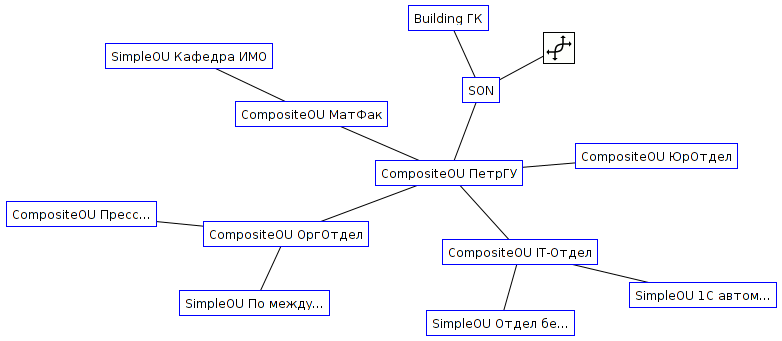
\includegraphics[scale=0.5]{figures/model_snapshot_org_petrsu}
  \caption{Пример организационной структуры модели Nest}
  \label{fig:model-snapshot-org}
\end{figure}


Запрос ``найти все вышестоящие отделы для всех \cl{CompositeOU} модели'' может быть
задан так
%Еще один пример на модели, приведенной на рис.~\ref{fig:model-snapshot-org}.
\query{compositeou.parent+}
и даст следующий результат:
\begin{center}
    \begin{tabular}{|l|l|}
	\hline
	\it{parent} & \it{parent}\\[5pt]
	\hline
	\hline
	\cl{null} & \cl{null} \\
	\hline
	ПетрГУ & \cl{null}\\
	\hline
	ПетрГУ & \cl{null}\\
	\hline
	ПетрГУ & \cl{null}\\
	\hline
	ОргОтдел & ПетрГУ \\
	\hline
    \end{tabular}
\end{center}

Если необходимо включить в запрос сам \cl{compositeou}, то для этого нужно
выполнять запрос
\query{compositeou.parent*},
который даст следующий результат:
\begin{center}
    \begin{tabular}{|l|l|l|}
	\hline
	\it{compositeou} & \it{parent} & \it{parent}\\[5pt]
	\hline
	\hline
	ПетрГУ & \cl{null} & \cl{null}\\
	\hline
	МатФак & ПетрГУ & \cl{null}\\
	\hline
	IT-Отдел & ПетрГУ & \cl{null}\\
	\hline
	ОргОтдел & ПетрГУ & \cl{null}\\
	\hline
	Пресс-Служба & ОргОтдел & ПетрГУ \\
	\hline
    \end{tabular}
\end{center}


Кроме того, класс \cl{CompositeOU} имеет свойство \cl{OUs}, которое является
коллекцией, состоящей из объектов \cl{AbstractOU}. Если необходимо
узнать всю иерархию организационных единиц для всех \cl{CompositeOU} модели,
то это можно сделать с помощью запроса
\query{compositeou.ous*}
, который вернет следующий результат: 
\begin{center}
    \begin{tabular}{|l|l|l|}
	\hline
	\it{compositeou} & \it{ous} & \it{ous}\\[5pt]
	\hline
	\hline
	ПетрГУ &  ЮрОтдел & \cl{null} \\
	\cline{2-3}
		    & ОргОтдел & По международным связям \\
	\cline{3-3}
		    &	       & Пресс-Служба \\
	\cline{2-3}
		    & IT-Отдел & Отдел безопасности\\
	\cline{3-3}
		    &	       & 1C автоматизация \\
	\cline{2-3}
		    & МатФак & Кафедра ИМО \\
	\hline
	ОргОтдел & По международным связям & \cl{null} \\
	\cline{2-3}
		& Пресс-Служба & \cl{null} \\
	\hline
	IT-Отдел & Отдел безопасности & \cl{null} \\
	\cline{2-3}
		& 1C автоматизация & \cl{null} \\
	\hline
	ЮрОтдел & \cl{null} & \cl{null} \\
	\hline
	Пресс-Служба & \cl{null} & \cl{null} \\
	\hline
	МатФак & Кафедра ИМО & \cl{null} \\
	\hline
    \end{tabular}
\end{center}



\subsubsection{Связанные элементы и рекурсивные ссылки}
\begin{figure}[hbt]
  \centering
  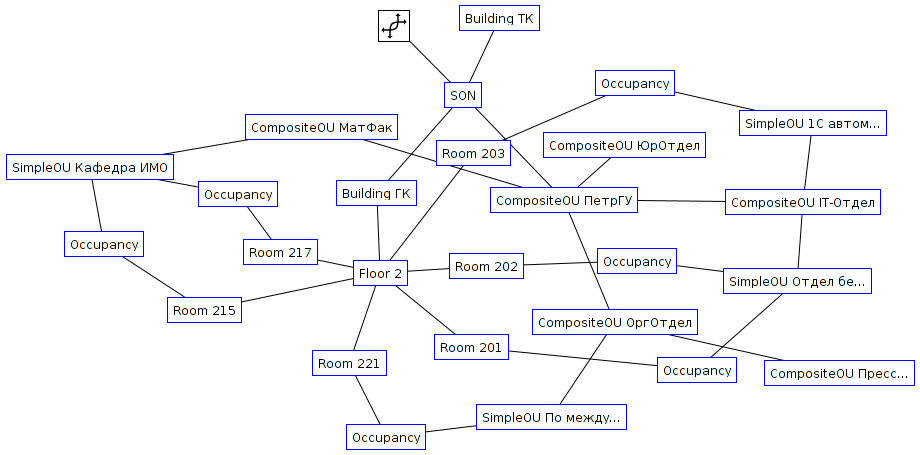
\includegraphics[scale=0.5]{figures/model_snapshot_org_spa_big}
  \caption{Пример организационной и пространственной структуры модели Nest}
  \label{fig:model-snapshot-org-spa}
\end{figure}

В запросах с рекурсивными ссылками и связанными элементами на 
последующих уровнях иерархии, связанные элементы будут указываться вместе
с последующим рекурсивным объектом. Например, запрос
\query{simpleou.parent* (room)}
на примере модели, изображенной на рис.~\ref{fig:model-snapshot-org-spa}, 
вернет результат приведенный в таблице~\ref{table:complex-query}.
\begin{table}[p]
  \centering
    \begin{tabular}{|l|l|l|l|}
	\hline
	\it{simpleou} & \it{parent,room} & \it{parent,room} & \it{room} \\[5pt]
	\hline
	\hline
	1C автоматизация & IT-Отдел & ПетрГУ & Room 201\\
	\cline{4-4}
		    &  &  & Room 202\\
	\cline{4-4}
		    &  &  & Room 203\\
	\cline{4-4}
		    &  &  & Room 215\\
	\cline{4-4}
		    &  &  & Room 217\\
	\cline{4-4}
		    &  &  & Room 221\\
	\cline{3-4}
		    &  & Room 201 & \\
	\cline{3-4}
		    &  & Room 202 & \\
	\cline{3-4}
		    &  & Room 203 & \\
	\cline{2-4}
		    & Room 203 & & \\
	\hline
	Отдел безопасности & IT-Отдел & ПетрГУ & Room 201\\
	\cline{4-4}
		    &  &  & Room 202\\
	\cline{4-4}
		    &  &  & Room 203\\
	\cline{4-4}
		    &  &  & Room 215\\
	\cline{4-4}
		    &  &  & Room 217\\
	\cline{4-4}
		    &  &  & Room 221\\
	\cline{3-4}
		    &  & Room 201 & \\
	\cline{3-4}
		    &  & Room 202 & \\
	\cline{3-4}
		    &  & Room 203 & \\
	\cline{2-4}
		    & Room 201 & & \\
	\cline{2-4}
		    & Room 202 & & \\
	\hline
	По международным связям & ОргОтдел & ПетрГУ & Room 201\\
	\cline{4-4}
		    &  &  & Room 202\\
	\cline{4-4}
		    &  &  & Room 203\\
	\cline{4-4}
		    &  &  & Room 215\\
	\cline{4-4}
		    &  &  & Room 217\\
	\cline{4-4}
		    &  &  & Room 221\\

	\cline{3-4}
		    &  & Room 221 & \\
	\cline{2-4}
				& Room 221 &  & \\
	\hline
	Кафедра ИМО & МатФак & ПетрГУ & Room 201\\
	\cline{4-4}
		    &  &  & Room 202\\
	\cline{4-4}
		    &  &  & Room 203\\
	\cline{4-4}
		    &  &  & Room 215\\
	\cline{4-4}
		    &  &  & Room 217\\
	\cline{4-4}
		    &  &  & Room 221\\
	\cline{3-4}
		    &  & Room 215 & \\
	\cline{3-4}
		    &  & Room 217 & \\
	\cline{2-4}
		    & Room 215 & & \\
	\cline{2-4}
		    & Room 217 & & \\
	\hline
    \end{tabular}
    \caption{результат запроса \itshape{\bfseries{simpleou.parent* (room)}}}
    \label{table:complex-query}

\end{table}

Обратите внимание, что \cl{room} привязываются как к самому \cl{simpleou}, так и к
его \cl{parent}, что согласуется с общей концепцией связанных элементов: элемент
на следующем уровне иерархии привязывается к последнему элементу предыдущего уровня
иерархии.

\subsection{Ограничения}
Язык позволяет задавать ограничения на элементы кортежа прямо в определении структуры кортежа.
Например, запрос
\query{room.number=``215''}
вернет список комнат, номером которых является значение ``215''.

Для организации сложных условий может использоваться: 
    \begin{itemize}\addtolength{\itemsep}{-0.7\baselineskip}
	\item логическое ``И'' (знак ``$\&\&$'' или слово {\itshape{\bfseries and}}),
	\item логическое ``ИЛИ'' (знак ``$||$'' или слово {\itshape{\bfseries or}}),
	\item отрицание (знак ``!''),
	\item круглые скобки для группировки сложных условий.
    \end{itemize}

В ограничениях могут использоваться следующие бинарные операции:
    \begin{itemize}\addtolength{\itemsep}{-0.7\baselineskip}
	\item ``='' --- равенство. 
%		Применимы к любым типам данных. 
		Обозначает одну и ту же величину 
		(т.е. 1 будет равно 1.0) или один и тот же объект.
	\item ``>'', ``>='', ``<'', ``<='' --- знаки категории ``больше-меньше''. 
%		Применимы к числовым и строковым типам.
	\item ``\symbol{"7E}'' --- знак регулярного выражения. 
%		Применим к строковым типам данных.
    \end{itemize}

Набор типов, к которым могут применяться бинарные операции, задается реализацией
данной спецификации. Однако, реализация должна поддерживать, по-крайней мере,
следующие представления данных:
    \begin{itemize}\addtolength{\itemsep}{-0.7\baselineskip}
	\item Строка.
	    \query{building.name=``ГК''}
	    Строка должна быть заключена в двойные кавычки. Внутри двойных кавычек может
	    использоваться любой символ. Чтобы использовать двойную кавычку, необходимо
	    ее экранировать с помощью обратного слеша (\symbol{"5C}), сам обратный слеш также
	    необходимо экранировать:
	    \query{building.name=``Building \symbol{"5C}``Main\symbol{"5C}''''}

	\item Число. Числа могут быть положительными, отрицательными, целыми и с плавающей точкой.
	    \query{floor.number>=1}

	\item Элемент запроса. Например, в запросе
	    \query{floor.number>=1} левая часть бинарной операции (\cl{floor.number}) является элементом.
	
	\item Ключевые слова \cl{true} и \cl{false} для возможности сравнения данных логического типа:
	    \queryexpl{Найти все маршрутизаторы сети}{device.forwarding=true}

	\item Ключевое слово \cl{nil} для обозначение элемента как не содержащего никакого значения:
	    \queryexpl{Найти все здания с заданным значением свойства \cl{name}}{building.name!=nil}

   \end{itemize}

Если типы правой и левой частей не совпадает, то пользователь должен получить сообщение
об ошибке. Например, в запросе
\query{floor.number=``IMO''}
поле \cl{number} класса \cl{Floor} имеет тип целое число. Сравнивая его со строкой,
пользователь должен получить сообщение об ошибке.






\subsubsection{Сложные ограничения}
ЯЗ позволяет задавать сложные ограничения как на одно свойство класса, так и на множество.
%Сложные условия можно использовать на одно свойство класса, 
Например в запросе
\queryexpl{Найти комнаты с номерами либо ``215'', либо ``217''}{room.number=(``215'' ``217'')}
указано несколько ограничений на одно свойство \cl{number}. Подразумевается, что эти значения
находятся в соотношении ``ИЛИ'', потому что при знаке $=$ логический оператор  ``И''
превращает данный запрос в бессмыслицу. Также логический оператор можно указать явно:
\query{room.number=(``215''~||~``217'')}


В предыдущем запросе знак ``='' можно переопределить следующим образом:
\queryexpl{Выбрать комнаты с номерами либо 215, либо начинающиеся с цифры 3}{room.number=(``215'' || \symbol{"7E} ``3.*'')}
Такая возможность может быть полезна, если необходимо ограничить значение свойства,
используя разные знаки соотношения:
\queryexpl{Выбрать этажи с первого по пятый}{floor.number(>=1~$\&\&$~<=5)}
Обратите внимание, что в том случае
если все знаки определены внутри скобок, указание знака перед скобками необязательно.

Если необходимо ограничение на несколько свойств одного объекта, то задавать его
нужно в скобках после точки. Например:
\queryexpl{Найти комнату с номером ``215'' и именем ``IMO\_215''}{room.(number=``215'' $\&\&$ name=``IMO\_215'')}

Приведем дополнительные примеры, демонстрирующие возможность определения сложных условия:
\query{
    room.(!number=``215'' $\&\&$ number \symbol{"7E} ``2.*'')
    \vspace{0.5cm}

    room.number(!=``215'' $\&\&$ \symbol{"7E} ``2.*'')
    \vspace{0.5cm}
    
    floor.number((>= 1 $\&\&$ <=5) || =10)
    \vspace{0.5cm}
	
    room.(number=``215'' \\
    \makebox[3em][r]{} $\&\&$ name=(``IMO\_215'' ``PMIK\_215'') \\
    \makebox[3em][r]{} $\&\&$ description=``Main room of the IMO'')
    \vspace{0.5cm}
    
    room.(number=``215'' \\
    \makebox[3em][r]{} $||$ (floor.number=2\\
    \makebox[3em][r]{} $\&\&$ description=``Main room of the IMO''))

}







\subsubsection{Вложенные обращения}
Возможно, что потребуется выбрать некоторое подмножество вложенного обращения. Для этого
это подмножество необходимо заключить в скобки:
\query{(room.floor).building.name=``ГК''}
Вышеприведенный запрос вернет список этажей в здании(\cl{building}) с именем ``ГК''. 
Обратите внимание, что результат этого запроса, может отличаться от результата запроса
\query{(floor).building.name=``ГК''}
В результат второго запроса войдут все этажи здания с именем ``ГК'', а в первый только те,
в которых имеются комнаты. Второй запрос будет эквивалентен запросу
\query{floor.building.name=``ГК''},
так как без указания скобок во вложенных обращениях подразумевается, что выбирается первый указанный 
элемент. Такое соглашение действует только при наличии условия, так как запрос 
\query{floor.building.name}
вернет имена зданий, в которых есть этажи, но запрос
\query{(floor.building).name}
уже вернет не имена, а сами объекты \cl{building}.

Во вложенных обращения также позволяется задавать ограничения на свойства. Например,
в запросе
\query{floor.(number(>1 $\&\&$ <4)).room}
будут выбраны комнаты на этажах с 1 по 4.

Еще примеры:
\queryexpl{Найти устойства на каждом из этажей, номер которого равен 1 и 
    на котором есть комната с номером ``215'' и именем ``IMO''}
    {room.(name=``IMO'' $\&\&$ number=``215'').floor.(number=1).device}
%\queryexpl{Предыдущий запрос эквивалентен следующему}
%    {device.(floor.number=1 $\&\&$ room.(name=``IMO'' $\&\&$ number=``2''))}
\queryexpl{Найти комнаты в здании главного корпуса}
    {building.(name=``ГК'').room}
\queryexpl{Предыдущий запрос эквивалентен следующему}
    {room.building.name=``ГК''}



\subsubsection{Выборка свойств}
Если необходимо выбрать не сам объект, а его свойство, но при этом задать ограничение на другое
свойство, то сделать это можно, указав нужное свойство в квадратных скобках:
\queryexpl{Выбрать имена комнат с номером ``215''}{room[name].number=``215''}

Однако, запись запроса ``выбрать номера комнат, начинающихся с 2'' выглядела бы
избыточной:
\query{room[number].number \symbol{"7E} ``2.*''},
поэтому ЯЗ позволяет задавать ограничение прямо в квадратных скобках:
\query{room[number \symbol{"7E} ``2.*'']}.

На одно свойство распространяются все правила, описанные выше. Примеры
\query{
    room[number=(``215'' ``217'')]
    \vspace{0.5cm}

    floor[number(>=1 $\&\&$ <=5)]
    \vspace{0.5cm}

    floor[number((>=1 $\&\&$ <=5) || =10)]
}


Однако, если в квадратных скобках указаны два или более свойства с условиями, то между 
ними подразумевается логические условие ``И'', т.е такой запрос
\query{room[number=``215'' name=``IMO215'']}
можно перевести на естественный язык как ``найти все комнаты с номером 215 и именем IMO215, 
при этом в результат включить только номера и имена этих комнат''.
Если необходимо задавать сложные условия по нескольким свойствам одного объекта, то тогда их необходимо вынести:
\query{room[number name].(number=``215'' || name=``IMO215'')}






\subsubsection{Связанные элементы}
Условие на элемент кортежа подразумевает собой следующее действие: каждый кортеж из полученного набора кортежей
проверяется на заданное ограничение. Таким образом запрос
\query{building (room.number=``215'')}
вернет все здания, а у здания только те комнаты, номером которых является ``215''. Если в здании нет комнаты с 
номером ``215'', то в этом случае список комнат у такого здания будет пуст, но само здание будет
включено в результат запроса. Для того чтобы получить
только те здания, которые имеют комнату с номером ``215'', а также указать список комнат этих зданий, необходимо
выполнить запрос:
\query{building.room.number=``215'' (room)}
Обратите внимание, что список комнат будет полным, там будут не только комнаты с номером ``215'' (однако этот список будет 
обязательно содержать комнату с номером ``215''). Чтобы выбрать здания, имеющие комнату с номером ``215'', и 
указать только такие комнаты, необходимо выполнить запрос:
\query{building.room.number=``215'' (room.number=``215'')}

Стоит помнить про то, что элемент на следующем уровне иерархии привязывается к 
последнему выбираемому элементу на предыдущем уровне иерархии. Поэтому
\queryexpl{\cl{floor} привязывается к \cl{building}}{building.device.room.number=``215'' (floor)}
\queryexpl{\cl{floor} привязывается к \cl{device}}{(building.device).room.number=``215'' (floor)}






\subsubsection{Рекурсивные ссылки}
К запросам с рекурсивными ссылками применимы все обозначенные выше правила.
Например, запрос
\query{simpleou.(name=``Кафедра ИМО'').parent+}
выдаст всю иерархию \cl{parent} только для тех \cl{simpleou}, имена которых равны значению ``Кафедра ИМО''.

Если задать ограничение на саму рекурсивную ссылку, то данное ограничение будет применяться к каждому
объекту из иерархии. В результат такого запроса попадут только те иерархии, в которых есть хотя бы
один объект удовлетворяющий ограничению.
%Также можно задать ограничение на саму рекурсивную ссылку:
Например, 
\query{simpleou.parent+.name=``МатФак''}
Данный запрос можно трактовать как для каждого простой организационной единицы получить 
все вышестоящий подразделения, имя одного из которых равно значению ``МатФак''. Результат
такого запроса на примере модели, изображенной на рис.~\ref{fig:model-snapshot-org}, 
будет выглядеть следующим образом:

\begin{center}
    \begin{tabular}{|l|l|}
	\hline
	\it{parent} & \it{parent}\\[5pt]
	\hline
	\hline
	МатФак & ПетрГУ \\
	\hline
    \end{tabular}
\end{center}




\subsection{Функции}
Для того чтобы позволить пользователю получать в качестве результата запроса уже
преобразованную в требуемый вид выборку из БД, в язык было введено понятие функции.
Возможности, которые есть у пользователя для реализации функции определяются
реализацией данной спецификации. Например, в ЯЗ4J функцию
можно реализовывать либо на чистом Java, объявляя ее как статический метод некоторого класса, 
либо на языке, который предоставляет возможность вызвать выполнение реализованного на нем
кода через Scripting API.%~\cite{Bosanac:2007:SJL:1406211}. 

В качестве одного из элементов результата запроса может быть использован
результат, который возвращает функция. Вызов функции выглядит следующим образом
\query{@funcn}

Функция может быть:
    \begin{itemize}\addtolength{\itemsep}{-0.7\baselineskip}
	\item частью структуры результата запроса\footnote{Здесь и далее для примеров используется функция
\cl{count}, которая в качестве аргумента принимает список, а возвращает количество элементов в списке.
Подробнее смотри в~\ref{std-funcs}}:
	    \queryexpl{Найти здания и подсчитать количество этажей в них}{building (@count(room))}
	\item запросом:
	    \query{@count(room)}
	\item вызвана в условии:
	    \queryexpl{Найти здания с количеством этажей больше 3}{building.(@count(room)>3)}
	\item параметром функции:
	    \query{@funcn(1, @anotherfuncn())}
    \end{itemize}





\subsubsection{Параметры}\label{func-param}
Параметры функции указываются в круглых скобках после имени функции через точку с запятой
\footnote{Использование точки с запятой, отличного от большинства языков программирования знака, 
использующих запятую, связано с тем, что одним из видом параметра может быть запрос на ЯЗ, 
в синтаксисе которого используется запятая.}:
\query{@funcn(par1; par2; par3)}
Параметром функции может быть: 
    \begin{itemize}\addtolength{\itemsep}{-0.7\baselineskip}
	\item строка, заключенная в двойные кавычки;
	\item число;
	\item логическое ``да'' (ключевое слово \cl{true}) или ``нет'' (ключевое слово \cl{false});
	\item ключевое слово \cl{nil}, обозначающее пустое значени;
	\item запрос.
%	\item результат вызова другой функции;
%	\item объект предметной области;
%	\item список объектов предметной области.
    \end{itemize}

В том случае если параметром функции является запрос, то в качестве значения
параметра будет передан результат данного запроса, т.е. либо элемент, либо
список кортежей. Например, в запросе
\queryexpl{Подсчитать количество комнат}{@count(room)}
параметром функции \cl{@count} является запрос 
\query{room}
Результатом его выполнения является список комнат (\cl{room}), который и будет
передан функции.

Если необходимо, чтобы функция вызывалась с каждым кортежем отдельно из списка
результата запроса, то для этого необходимо в начале запроса-параметра
указать модификатор ``\#'':
\query{@funcn(\#room)}


Если функция находится на не первом уровне иерархии, то запросы-параметры
будут выполняться относительно последнего элемента предыдущего уровня иерархии.
Например, в запросе 
\query{building (@count(room))}
Список комнат (\cl{room}), переданный в функцию \cl{@count} будет формироваться относительно
здания(\cl{building}), т.е. данный запрос выведет список зданий и количество комнат в них.

В запросе
\query{building (floor, room (@count(device)))}
функция \cl{@count} будет подсчитывать количество устройств(\cl{device}) относительно комнаты(\cl{room}), т.е.
запрос выведет количество устройств в комнате. 

Если необходимо, чтобы на не первом уровне иерархии запрос выполнялся независимо от предыдущего уровня,
то в начале запроса необходимо указать модификатор \cl{\%}:
\query{building (@funcn(\%room))}
В приведенном выше запросе в функцию \cl{@funcn} будет передан весь список объектов
\cl{room}.

%Будьте осторожны, используя одновременно два модификатора в запросах с вызовом функции и 
%списком связанных элементов в качестве параметра на не первом уровне иерархии кортежа.
%В запросе
%\query{building (@funcn(\%\#room))}
%для каждого объекта \cl{building} будет вызвана функцию \cl{@funcn} с каждым
%объектом \cl{room}.

Использование одновременно двух модификаторов запрещено.







\subsubsection{Рассогласованность по параметрам функции}
Запрос называется рассогласованным по параметрам функции, если в нем вызывается
функция, для которой невозможно определить с каким набором параметров следует вызывать данную функцию.
Рассмотрим пример:
\query{@funcn(\#building; \#room)}
В данном запросе функция вызывается с двумя параметрами, значением которых является
выполнение запросов
\query{building}
и
\query{room}
Однако, модификатор \cl{\#} говорит о том, что в функцию необходимо передавать не весь результат
запроса, а каждый кортеж в отдельности. Таким образом, в 
нашем примере непонятно с какими кортежами из результатов запросов-параметров нужно вызывать
функцию. Может показаться, что проблема решается путем простого вызова функции с кортежами из результатов 
запросов-параметров по порядку. Однако, непонятно как действовать в том случае, если 
количество этих кортежей различно. Поэтому ЯЗ не допускает рассогласованности по параметрам функции.

%Рассмотрим пример частично рассогласованного запроса по параметрам функции. В таком запросе
%существет возможность определить






\subsubsection{Стандартная библиотека функций}\label{std-funcs}
Реализация данной спецификации может предоставить любой набор функции для работы с 
данными запроса. Однако, этот набор должен содержать, по крайней мере, следующие
функции:
\begin{description}
    \item [avg] --- вычисляет среднее значение элементов списка-аргумента.\\
	{\it Входные данные:} набор кортежей, состоящих из одного элемента, над которым
			    реализация позволяет производить арифметические операции.\\
	{\it Результат:} значение выражения $$\frac{\sum_{i=1}^n e_i}{n}$$, 
		    где $e_i$ --- значение элемента $i$-го кортежа, 
		    $n$ --- количество кортежей.
    \item [count] --- подсчитывает количество элементов в списке.\\
	{\it Входные данные:} список кортежей.\\
	{\it Результат:} количество элементов в списке-аргументе.
    \item [first] --- возвращает первый кортеж из списка-аргумента.\\
	{\it Входные данные:} список кортежей.\\
	{\it Результат:} первый кортеж из списка-аргумента.
    \item [last] --- возвращает последний кортеж из списка-аргмента.\\
	{\it Входные данные:} список кортежей.\\
	{\it Результат:} последний кортеж из списка-аргумента.
%    \item [distinct] возвращает тольк\\
%	{\it Входные данные:} \\
%	{\it Результат:}
    \item [max] --- возвращает максимальное значение из элементов списка-аргумента.\\
	{\it Входные данные:} набор кортежей, состоящих из одного элемента, над которым
			    реализация позволяет производить операцию сравнения.\\
	{\it Результат:} максимальное значение из элементов списка-аргумента.
    \item [min] --- возвращает минимальное значение из элементов списка-аргумента.\\
	{\it Входные данные:} набор кортежей, состоящих из одного элемента, над которым
			    реализация позволяет производить операцию сравнения.\\
	{\it Результат:} минимальное значение из элементов списка-аргумента.
    \item [sum] --- возвращает сумму значений элементов списка-аргумента.\\
	{\it Входные данные:} набор кортежей, состоящих из одного элемента, над которым
			    реализация позволяет производить арифметическую операцию сложения.\\
	{\it Результат:} сумма значений элементов списка-аргумента.
\end{description}


\subsection{Группировка}
\begin{center}
\end{center}
%Одной из основных особенностей ЯЗ является то, что он позволяет группировать
%связанные между собой объекты (см. подробнее~\ref{tied_queries}).
Часто бывает необходимым передать в функцию в качестве параметра список объектов сгруппированных
относительно другого набора объектов. Количество вызовов функции в этом случае будет соответствовать
количеству объектов второго набора.
%обрабатывать объекты сгруппировав их относительно других объектов. 
Часть таких возможностей обеспечивается вызовом функции на не первом уровне 
иерархии запроса (см. подробнее в~\ref{func-param}). Например, в запросе
\query{building (@count(room))}
список объектов \cl{room} формируется относительно объекта \cl{building},
находящегося на более высоком уровне иерархии. Таким образом мы можем группировать
списки, которые передаются в функцию.

Однако, идеология такого подхода несколько отличается от группировки, так как 
подразумевает под собой связь между объектами модели, поэтому этот подход
не позволяет, во-первых, не включать в результат объект более
высокого уровня иерархии, а во вторых группировать не относительно объекта, а 
относительно свойства объекта. Чтобы решить эти проблемы в ЯЗ был
введен специальный модификатор ``:'', который разделяет имя класса, объекты которого будут группироваться,
и определение класса или свойства класса, относительно которого будет происходить группировка.

%Вначале рассмотрим группировку на уровне запроса, а затем
Рассмотрим следующий пример:
\query{floor:number}
Результат данного запроса будет состоять из кортежей, элементом которых будет
список объектов класса \cl{floor}. У всех объектов \cl{floor} в списке будет
один и тот же номер, так как запрос подразумевает то, что объекты \cl{floor}
должны быть сгруппированы по поле \cl{number}.

Если в запросе указывается необходимость связать элемент со списком сгруппированных объектов,
то в набор связанных объектов попадут все объекты, которые связаны с объектами из списка
сгруппированных объектов.
Например, в запросе
\query{floor:number (@count(room))}
объекты класса \cl{room} будут связываться с объектами класса \cl{floor}, сгруппированными относительно свойства
\cl{number}. Таким образом, с точки зрения модели в функцию \cl{count} будет передаваться набор комнат, находящихся
на этажах с одинаковыми номерами.

Группировать можно как по свойству класса, так и по связанному с классом другому классу.
Например, результатом запроса
\query{room:building}
будут списки комнат (\cl{room}), находящихся в одном и том же здании (\cl{building}).
Приоритет поиска отношений между группируемым классом и определенем группировки
точно такой же как и при поиске связей (подробнее см. в~\ref{simple-select}).



\subsection{Сортировка}
Чтобы определить порядок, в котором будут располагаться 
выбираемые объекты, необходимо после имени класса
в структуре результата запроса указать в фигурных скобках набор полей и способ 
(для этого используются модификаторы \cl{asc} (по возрастанию) и \cl{desc} (по убыванию))
сортировки. Например, в запросе
\query{room\{desc:number\}}
кортежи с объектами \cl{room} будут отсортированы по полю \cl{number} в порядке 
убывания. 

Набор типов, по которым пользователь сможет задавать сортировку,
определяется реализацией данной спецификации.  Если тип выбираемого объекта или свойства объекта
определен в наборе, который поддерживается реализацией для сортировки, то достаточно указать порядок сортировки. 
Например, в запросе 
\query{room.number\{asc\}}
кортежи со строковыми значениями полей \cl{number} объектов \cl{room} будут
отсортированы по возрастанию.

Также можно задать несколько полей, по которым необходимо произвести сортировку. 
Например, объекты \cl{room} в результате запроса
\query{room\{desc:name asc:number\} }
будет вначале отсортирован по полю \cl{name} по убыванию, в случае если значения
\cl{name} совпадают, то затем по полю \cl{number} в порядке возрастания.

Если для порядка используется один модификатор для нескольких подряд идущих полей, 
то эти поля можно указывать после модификатора через запятую. Например:
\query{
    room\{desc:number,name\}\\
    room\{desc:number,name asc:id\}\\
    room\{asc:floor.number desc:number,name asc:id\}
}

Если сортировка применяется к элементу, находящемуся на не первом уровне иерархии, то
сортировка объектов производится внутри каждого кортежа по отдельности. Например, каждый
кортеж результата запроса
\query{building (room\{asc:number\})}
будет состоять из здания(\cl{building}) и набора комнат (\cl{room}), принадлежащих этому
зданию. Кроме того, этот набор комнат будет отсортирован в порядке возрастания (благодаря
модификатору \cl{asc}) по полю \cl{number} объекта \cl{room}.




\subsection{Настройка}
